\documentclass[11pt]{article}

\usepackage[margin=1.1in]{geometry}
\usepackage{amsmath, amssymb, amsthm}
\usepackage{tikz}
\usetikzlibrary{arrows.meta, positioning, decorations.pathreplacing}
\usepackage{booktabs}
\usepackage{array}

\newtheorem{claim}{Claim}

\title{Differential Operators on a Graph\\[4pt]
\large A theory guide for the graph engine}
\author{Komahan Boopathy}
\date{}

\begin{document}
\maketitle

\begin{abstract}
\noindent
A mesh is a graph: cells are vertices, faces are edges. This note
shows that once a problem lives on a graph, every differential
operator a partial differential equation needs -- first derivative,
second derivative, any order, curl, and each operator's adjoint -- is
built from three elementary steps, each of which is one walk over the
edges. A solver for a physical problem then writes no loops of its
own. It chooses operators, hands them coefficients, and the graph
engine does the rest. Every claim made here is proved by arithmetic
short enough to check by hand, and each construction is drawn before
it is written.
\end{abstract}

\section{The one-line law, and where this note fits}

The engine rests on one sentence: split a graph into parts, work on
the parts, put the answer back together.
\[
G' \;=\; P^{-1}\bigl(A\,(P(G))\bigr)
\]
$P$ is the partitioner, $P^{-1}$ the assembler, and $A$ an operation.
This note is about the operations $A$: the ones that turn a field of
values into its derivatives. When these exist, a solver for a
physical problem -- heat spreading through a plate, a quantity
carried along a flow -- is nothing but a \emph{choice} of operators
and coefficients. The physics chooses; the graph computes. That
division of labour is the point of the whole design, and
section~\ref{sec:delegation} spells it out.

\section{Graphs and fields}\label{sec:graphs}

A graph is vertices joined by edges. Every edge has a tail and a
head, so every edge points somewhere. An edge may also have a tail
and \emph{no} head: it starts at a vertex and stops. That is how a
boundary is written -- a face on the outside of a mesh touches one
cell only, and no imaginary cell is invented beyond it.

\begin{center}
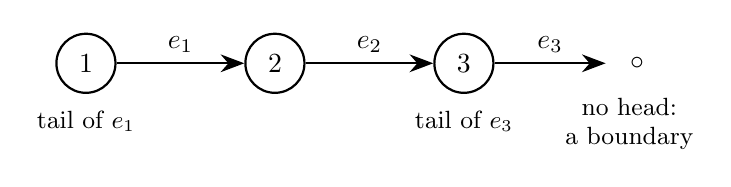
\begin{tikzpicture}[
  v/.style={circle, draw, thick, minimum size=7.5mm, inner sep=0pt},
  e/.style={-{Stealth[length=3mm]}, thick},
  scale=1.0]
  \node[v] (1) at (0,0)   {$1$};
  \node[v] (2) at (2.4,0) {$2$};
  \node[v] (3) at (4.8,0) {$3$};
  \draw[e] (1) -- node[above]{$e_1$} (2);
  \draw[e] (2) -- node[above]{$e_2$} (3);
  \draw[e] (3) -- node[above]{$e_3$} (6.6,0);
  \node at (7.0,0) {$\circ$};
  \node[below=1mm of 1] {\small tail of $e_1$};
  \node[below=1mm of 3] {\small tail of $e_3$};
  \node at (6.9,-0.55) {\small no head:};
  \node at (6.9,-0.95) {\small a boundary};
\end{tikzpicture}
\end{center}

A \emph{vertex field} is a value per vertex; call the values $q_v$.
An \emph{edge field} is a value per edge; call the values $z_e$.
Nothing more is needed. (A reader who knows the exterior-calculus
literature may recognise these as $0$- and $1$-cochains; the names
are never needed again.)

Each edge also carries a length $h_e$, the spacing between its two
ends, and each vertex carries a measure $m_v$ -- on a mesh, the
volume of its cell. On the uniform chains used for the proofs below,
$h_e = h$ and $m_v = h$ everywhere.

\section{Three elementary steps}\label{sec:steps}

Everything in this note is built from three ways of moving values
between vertices and edges. Two go from vertices to edges; one comes
back.

\begin{center}
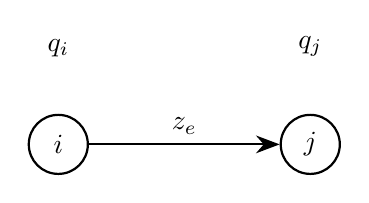
\begin{tikzpicture}[
  v/.style={circle, draw, thick, minimum size=7.5mm, inner sep=0pt},
  e/.style={-{Stealth[length=3mm]}, thick}, scale=1.0]
  \node[v] (i) at (0,0)   {$i$};
  \node[v] (j) at (3.2,0) {$j$};
  \draw[e] (i) -- node[above]{$z_e$} (j);
  \node[above=6mm of i] {$q_i$};
  \node[above=6mm of j] {$q_j$};
\end{tikzpicture}
\end{center}

\paragraph{The edge average step $S$} puts on each edge the mean of $q$
along the edge -- its integral over the edge divided by the edge's
length, which for a straight-line $q$ is exactly the average of the
two end values -- or, when a direction matters, the same integral
read at one end, chosen by the sign of the coefficient:
\[
(Sq)_e = \tfrac{1}{2}(q_i + q_j)
\qquad\text{or}\qquad
(Sq)_e = q_i \ \text{ or } \ q_j .
\]

\paragraph{The difference step $G$} puts on each edge the difference
of its two end values over the spacing:
\[
(Gq)_e = \frac{q_j - q_i}{h_e}.
\]
This is the slope of $q$ along the edge.

\paragraph{The incidence step $D$} brings edge values back to the
vertices. Each vertex adds up the values on edges leaving it, minus
the values on edges entering it, and divides by its measure:
\[
(Dz)_v = \frac{1}{m_v}\Bigl(
  \sum_{\text{edges leaving } v} z_e \;-\;
  \sum_{\text{edges entering } v} z_e \Bigr).
\]
An edge with no head contributes to its tail alone.

\begin{center}
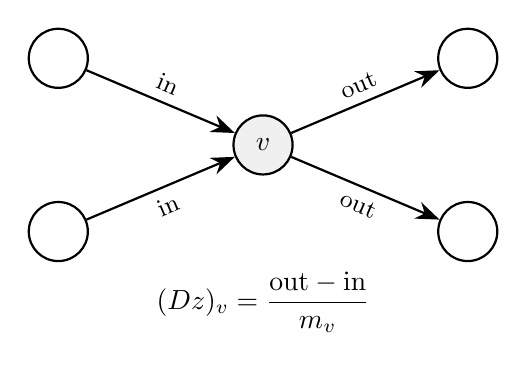
\begin{tikzpicture}[
  v/.style={circle, draw, thick, minimum size=7.5mm, inner sep=0pt},
  e/.style={-{Stealth[length=3mm]}, thick}, scale=1.0]
  \node[v] (a) at (-2.6,1.1)  {};
  \node[v] (b) at (-2.6,-1.1) {};
  \node[v, fill=black!6] (i) at (0,0) {$v$};
  \node[v] (c) at (2.6,1.1)  {};
  \node[v] (d) at (2.6,-1.1) {};
  \draw[e] (a) -- node[above, sloped]{\small in} (i);
  \draw[e] (b) -- node[below, sloped]{\small in} (i);
  \draw[e] (i) -- node[above, sloped]{\small out} (c);
  \draw[e] (i) -- node[below, sloped]{\small out} (d);
  \node at (0,-2.0) {$\displaystyle (Dz)_v = \frac{\text{out} - \text{in}}{m_v}$};
\end{tikzpicture}
\end{center}

At a boundary the missing end needs a value. The operator stores one
(a single number, or one per boundary edge), and $S$ and $G$ use it
in place of the value that is not there. This is where a boundary
condition's \emph{data} enters; the operator itself does not change.

One convention to fix now, because two are in use. The incidence
step above is
\emph{out minus in}; it makes the derivative formulas of the next
section come out with their textbook signs. The balance operation in
the engine counts the other way -- in minus out -- because a balance
counts what a vertex \emph{gains}. The two directions differ by a sign and
both are stated where they appear. Nothing deeper is going on.

\section{Any order, by repeating the steps}\label{sec:orders}

Apply the steps in alternation and the derivatives appear in
sequence. On the chain below, with uniform spacing $h$ and measure
$m = h$:

\begin{center}
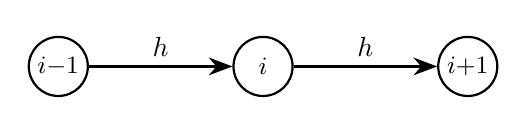
\begin{tikzpicture}[
  v/.style={circle, draw, thick, minimum size=7.5mm, inner sep=0pt},
  e/.style={-{Stealth[length=3mm]}, thick}, scale=1.0]
  \node[v] (1) at (0,0)  {\small$i{-}1$};
  \node[v] (2) at (2.6,0){\small$i$};
  \node[v] (3) at (5.2,0){\small$i{+}1$};
  \draw[e] (1) -- node[above]{$h$} (2);
  \draw[e] (2) -- node[above]{$h$} (3);
\end{tikzpicture}
\end{center}

\medskip
\begin{center}
\begin{tabular}{@{}llll@{}}
\toprule
order & recipe & result at an interior vertex & name \\
\midrule
0 & $c\,q$              & $c\,q_i$ & the term itself \\
1 & $D\,S\,q$           & $c\,\dfrac{q_i - q_{i-1}}{h}$ & first derivative \\[6pt]
2 & $D\,G\,q$           & $c\,\dfrac{q_{i+1} - 2q_i + q_{i-1}}{h^2}$ & second derivative \\[6pt]
3 & $D\,G\,D\,S\,q$     & (the stencil widens) & third \\
4 & $D\,G\,D\,G\,q$     & fourth difference over $h^4$ & fourth \\
$n$ & one more step     & reaches $n$ rings of neighbours & $n$-th \\
\bottomrule
\end{tabular}
\end{center}
\medskip

The recipes on the edge side read the same way: order $0$ is $S\,q$,
order $1$ is $G\,q$, and order $n$ applies $G$ to the vertex result
of order $n-1$. The coefficient $c$ is applied once, at the innermost step -- the
first moment the values land on the edges -- which is what lets a
coefficient vary edge by edge. (The order-$2$ recipe is what the literature calls the graph
Laplacian; the name is not needed to use it.)

Each step consults only an edge's two ends, so each step widens the
reach of the answer by exactly one ring of neighbours: the order-$n$
operator sees precisely the vertices a walk of $n$ edges can reach.
Arbitrary order is therefore one integer and a loop -- nothing about
a graph makes order 7 harder than order 2.

\begin{claim}[The second derivative is exact on a parabola]
Take the uniform chain with $q_v = v^2$ and $c = 1$. The whole
computation fits in three lines. The difference step gives, on the
two edges at $i$,
\[
(Gq)_{(i-1,i)} = \frac{i^2 - (i-1)^2}{h} = \frac{2i-1}{h},
\qquad
(Gq)_{(i,i+1)} = \frac{(i+1)^2 - i^2}{h} = \frac{2i+1}{h},
\]
and the incidence step subtracts them and divides by $m=h$:
\[
(DGq)_i = \frac{1}{h}\Bigl(\frac{2i+1}{h} - \frac{2i-1}{h}\Bigr)
        = \frac{2}{h^2}.
\]
In the chain's coordinates $x = vh$ this is the statement that the
second derivative of $x^2$ is $2$, exactly. On a straight line $q_v = av + b$ the
same two lines give zero. \qed
\end{claim}

\begin{claim}[Order four is exact on $x^4$]
With $q_v = v^4$ and $h = 1$, one application of $DG$ gives, by the
same arithmetic,
\[
(DGq)_i = (i+1)^4 - 2i^4 + (i-1)^4 = 12 i^2 + 2 ,
\]
and applying $DG$ once more to $12 i^2 + 2$ gives, by the parabola
claim, $12 \cdot 2 = 24$: the fourth derivative of $x^4$, exactly, at
every vertex two rings inside the boundary. \qed
\end{claim}

Odd orders above one mix a one-sided step with centred ones, so they
match a hand-computed stencil rather than a single calculus formula;
the test suite checks them against that stencil.

\section{Coefficients that vary: the non-uniform case}
\label{sec:weights}

Nothing above requires the coefficient, the spacing, or the boundary
value to be one number. Give every edge its own:
\[
z_e = c_e\,\frac{q_j - q_i}{h_e},
\qquad
(Dz)_v = \frac{1}{m_v}\bigl(\text{out} - \text{in}\bigr),
\]
and order 2 becomes the operator
$\mathrm{div}\,(k\,\mathrm{grad}\,q)$ with a conductivity that varies
in space -- each edge carries its own $c_e$. The uniform case is the
special case of equal values.

This is also precisely the finite-volume method, which is why this
machinery replaces the hand-written assembler. Read the dictionary:

\medskip
\begin{center}
\begin{tabular}{@{}lll@{}}
\toprule
mesh quantity & graph home & used by \\
\midrule
cell               & vertex            & everything \\
interior face      & edge with a head  & $S$, $G$, $D$ \\
boundary face      & edge, no head     & boundary values \\
cell volume $V_v$  & vertex measure $m_v$ & the incidence step \\
face area $A_e$ and conductivity $k_e$
                   & edge coefficient $c_e = k_e A_e$ & the difference step \\
centre-to-centre distance $d_e$
                   & edge spacing $h_e$ & the difference step \\
\bottomrule
\end{tabular}
\end{center}
\medskip

With those entries, the order-2 vertex operator at cell $v$ reads
\[
\frac{1}{V_v}\sum_{\text{faces of } v} \pm\, k_e A_e\,
\frac{q_{\text{other}} - q_v}{d_e},
\]
which is the finite-volume discretisation of
$\mathrm{div}(k\,\mathrm{grad}\,q)$, term for term. The engine never
needs to know it is doing finite volume; the mesh hands the graph its
geometry, and the formula falls out.

\section{From operators to equations}\label{sec:pdes}

A transport equation,
\[
\frac{\partial q}{\partial t}
 = -\,\mathrm{div}(u\,q) \;+\; \mathrm{div}(k\,\mathrm{grad}\,q)
   \;+\; s,
\]
asks for exactly three configured operators and a source: an order-1
vertex operator with coefficient $u$ (the sign of $u$ choosing the
sampled end -- values are taken from the side the flow comes from),
an order-2 vertex operator with coefficient $k$, and an order-0 term
for $s$. The engine's balance operation sums such terms and a time
integrator marches the result. Boundary conditions are not special
operators: they are the stored values at the headless edges,
per-edge when the boundaries differ.

Signs deserve one honest sentence. Physical laws carry their own sign
conventions -- a flux runs \emph{down} a gradient, so a model writes
its diffusion coefficient with the sign its law requires. The graph
layer computes derivatives; which sign a term enters an equation with
is the model's statement, made in the model's own class.

\section{Going around instead of along: curl}\label{sec:curl}

The derivative along edges is not the only derivative. Around a loop
of edges there is another one: add up the edge values as you walk the
loop. If the values came from differences of a vertex field, the walk
telescopes to nothing; if the values circulate, it does not. That sum
is the curl.

Where does it live? A loop of edges bounds a face, and a face is not
a vertex or an edge -- but \emph{which edge borders which face} is
itself a graph. Build it: one vertex for every edge of the original
graph, one vertex for every face, and a connection wherever an edge
borders a face, carrying $+1$ if the edge agrees with the direction
of the walk around the face and $-1$ if it opposes it.

\begin{center}
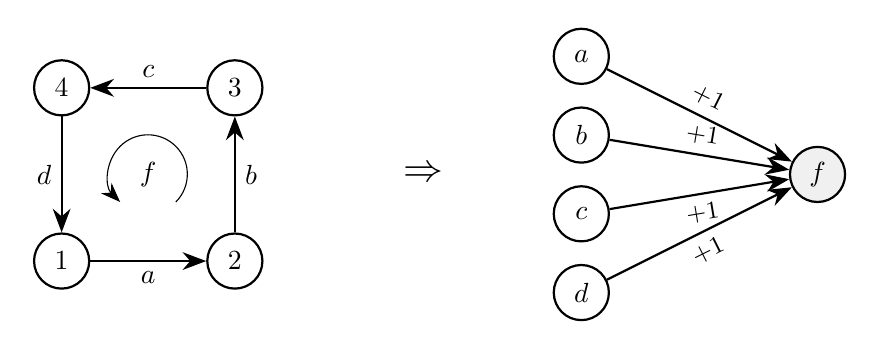
\begin{tikzpicture}[
  v/.style={circle, draw, thick, minimum size=7mm, inner sep=0pt},
  e/.style={-{Stealth[length=3mm]}, thick}, scale=1.0]

  \node[v] (1) at (0,0)   {$1$};
  \node[v] (2) at (2.2,0) {$2$};
  \node[v] (3) at (2.2,2.2) {$3$};
  \node[v] (4) at (0,2.2)  {$4$};
  \draw[e] (1) -- node[below]{$a$} (2);
  \draw[e] (2) -- node[right]{$b$} (3);
  \draw[e] (3) -- node[above]{$c$} (4);
  \draw[e] (4) -- node[left]{$d$}  (1);
  \node at (1.1,1.1) {$f$};
  \draw[-{Stealth[length=2.5mm]}] (1.45,0.75) arc (-45:225:0.5);

  \node at (4.6,1.1) {\Large$\Rightarrow$};

  \node[v] (ea) at (6.6,2.6) {$a$};
  \node[v] (eb) at (6.6,1.6) {$b$};
  \node[v] (ec) at (6.6,0.6) {$c$};
  \node[v] (ed) at (6.6,-0.4){$d$};
  \node[v, fill=black!6] (f) at (9.6,1.1) {$f$};
  \draw[e] (ea) -- node[above, sloped]{\small$+1$} (f);
  \draw[e] (eb) -- node[above, sloped]{\small$+1$} (f);
  \draw[e] (ec) -- node[below, sloped]{\small$+1$} (f);
  \draw[e] (ed) -- node[below, sloped]{\small$+1$} (f);
\end{tikzpicture}
\end{center}

\noindent
On this second graph, the edge values of the original become a vertex
field, and the incidence step -- the same $D$ as everywhere in this note,
with the $\pm 1$ as its per-edge coefficients -- collects the walk
around each face. The curl is the incidence step on the border graph.
Nothing new is built.

\begin{claim}[The curl of a difference field is zero]
Walk the square: the edge values of a difference field are
$z_a = q_2 - q_1$, $z_b = q_3 - q_2$, $z_c = q_4 - q_3$,
$z_d = q_1 - q_4$. Their sum,
\[
(q_2 - q_1) + (q_3 - q_2) + (q_4 - q_3) + (q_1 - q_4) = 0,
\]
cancels term against term, for any values $q$. \qed
\end{claim}

A field that circulates -- say $z_a = z_b = z_c = z_d = 1$ -- sums to
$4$, not zero, so the construction detects rotation, which is its
job. The same move repeats upward: loops of faces bound volumes, and
their border relation is again a graph, for whoever needs it.

\section{Adjoints: the same walk, backwards}\label{sec:adjoints}

Every operator here is a walk over the edges. Its adjoint -- the
operator $A^{\!*}$ with
$\sum_v (Aq)_v\,p_v = \sum_v q_v\,(A^{\!*}p)_v$, the thing an
adjoint (sensitivity) solver consumes -- is the same walk with every
edge reversed.

\begin{center}
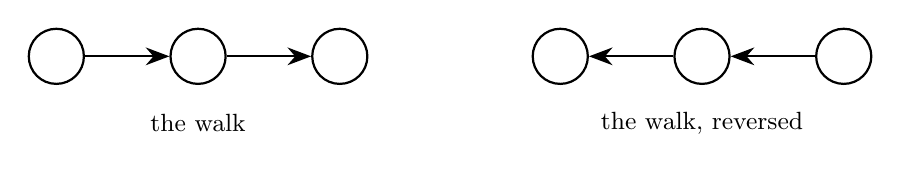
\begin{tikzpicture}[
  v/.style={circle, draw, thick, minimum size=7mm, inner sep=0pt},
  e/.style={-{Stealth[length=3mm]}, thick}, scale=1.0]
  \node[v] (1) at (0,0)   {};
  \node[v] (2) at (1.8,0) {};
  \node[v] (3) at (3.6,0) {};
  \draw[e] (1) -- (2);
  \draw[e] (2) -- (3);
  \node at (1.8,-0.85) {\small the walk};
  \node[v] (4) at (6.4,0)  {};
  \node[v] (5) at (8.2,0)  {};
  \node[v] (6) at (10.0,0) {};
  \draw[e] (5) -- (4);
  \draw[e] (6) -- (5);
  \node at (8.2,-0.85) {\small the walk, reversed};
\end{tikzpicture}
\end{center}

To see it, take the plain sums ($h = m = 1$ keeps the arithmetic
bare; weights ride along unchanged). Pair a vertex field $p$ with an
incidence step:
\[
\sum_v p_v\,(Dz)_v
 = \sum_e z_e\,\bigl(p_{\text{tail}(e)} - p_{\text{head}(e)}\bigr)
 = -\sum_e z_e\,(Gp)_e .
\]
The first equality is only a change of viewpoint: instead of walking
vertices and asking which edges touch each one, walk edges and ask
which vertices each one touches -- every edge hands $+z_e$ to its
tail's row and $-z_e$ to its head's row. So
\[
D^{\!*} = -\,G, \qquad G^{\!*} = -\,D,
\]
and the one-sided average step's adjoint returns each value, unsigned, to the
end it sampled. Reversing every edge swaps tail with head, which
swaps out with in, which is exactly these transposes: the reverse
walk.

Adjoints of compositions run the transposed steps in reverse order.
Two consequences follow immediately:
\[
(DG)^{\!*} = G^{\!*}D^{\!*} = (-D)(-G) = DG ,
\]
so the second-derivative operator is its own adjoint whenever the
same per-edge coefficients sit on both steps -- and the order-1
operator's adjoint samples from the \emph{other} end and counts the
other way, which is precisely the reversed-flow operator a
sensitivity solve requires. The engine gets both by a flag: run the
walk backwards. No second implementation exists to drift out of
agreement with the first.

\section{Cut into parts, the operators do not notice}
\label{sec:parts}

The engine's three laws state that partitioning is invisible to
results:
\[
P^{-1}(P(G)) = G, \qquad
P^{-1}(P(G,D)) = (G,D), \qquad
A(G,D) = P^{-1}\bigl(A(P(G,D))\bigr).
\]
The steps of this note obey the third law for the same reason the
balance does: each step reads an edge's two ends, and a part carries
-- as its borrowed vertices -- every end its owned edges need. A part
computes its owned share exactly; assembly collects owned values
only; the pieces sum to the whole.

One reduction subtlety travels with partitioning and is worth
restating. A quantity like an average must be combined across parts
\emph{unfinished}: two parts averaging $2$ and $7$ combine to $4$ --
twenty over five -- not $4.5$. The engine's reductions carry their
running sums and counts together and divide once, at the end.

\section{What a physics class actually does}\label{sec:delegation}

Everything above belongs to the engine. A model of a physical problem
now delegates:

\begin{enumerate}
  \item \textbf{choose operators} -- which orders appear in its
        equation;
  \item \textbf{fill coefficients} -- from geometry
        ($c_e = k_e A_e$, $h_e = d_e$, $m_v = V_v$) and, for a
        nonlinear law, from the current state, refreshed each
        evaluation;
  \item \textbf{state its signs} -- its own flux convention, in its
        own class;
  \item \textbf{set boundary values} -- per headless edge, from its
        boundary conditions.
\end{enumerate}

\noindent
Worked example, heat in a plate: $\partial q/\partial t =
\mathrm{div}(k\,\mathrm{grad}\,q)$ with insulated boundaries. The
model builds one order-2 vertex operator; fills $c_e = k_e A_e$,
$h_e = d_e$, $m_v = V_v$ from the mesh; sets each boundary edge's
stored value equal to its cell's value (no difference across the
boundary, so no flow); and hands the operator to the balance and the
balance to a time integrator that already exists. The model contains
no loop over cells or faces. That absence is the design goal.

Three pieces complete the full replacement of the old hand-written
assembler, all already mapped: the mesh migration that feeds the
coefficient arrays from stored geometry; state-dependent coefficients
recomputed per evaluation (the delegation point for nonlinear laws);
and systems of equations, which ride on the fields'
\texttt{num\_components} unchanged.

\section{The dictionary}\label{sec:dictionary}

\begin{center}
\begin{tabular}{@{}lll@{}}
\toprule
in this note & in the engine & kind \\
\midrule
vertex field $q$      & \texttt{vertex\_field}                & type \\
edge field $z$        & \texttt{edge\_field}                  & type \\
edge average step $S$ & \texttt{average\_step}                & kernel \\
difference step $G$   & \texttt{difference\_step}             & kernel \\
incidence step $D$    & \texttt{incidence\_step}              & kernel \\
operator, edge side   & \texttt{edge\_differential\_operator} & type \\
operator, vertex side & \texttt{vertex\_differential\_operator} & type \\
order $n$             & \texttt{order}                        & component \\
$c$, $c_e$            & \texttt{coefficient}, \texttt{coefficients(:)} & component \\
$h$, $h_e$            & \texttt{spacing}, \texttt{spacings(:)} & component \\
$m_v$                 & \texttt{measures(:)} on the vertex side & component \\
boundary value        & \texttt{boundary\_value}, \texttt{boundary\_values(:)} & component \\
the reverse walk      & \texttt{adjoint} flag                 & component \\
order 1, edge side    & \texttt{gradient(...)}                & constructor \\
order 0, edge side    & \texttt{interpolation(...)}           & constructor \\
order 1, vertex side  & \texttt{divergence(...)}              & constructor \\
order 2, vertex side  & \texttt{laplacian(...)}               & constructor \\
sum of terms          & \texttt{balance}                      & type \\
\bottomrule
\end{tabular}
\end{center}

\bigskip
\noindent
Every claim in this note reappears in \texttt{test/graph-contract} as
a check with the same numbers: the parabola's $2$, the fourth power's
$24$, the average's $4$-not-$4.5$, the square loop's $0$ -- and its
nonzero companion for a circulating field, because a check that
cannot fail proves nothing.

\end{document}
